\documentclass[journal,twoside]{IEEEtran}
% Updated from the supplied Overleaf source; Ethereum registry measurements added 2026-10-26.
\usepackage{cite}
\usepackage{amsmath,amssymb}
\usepackage{graphicx}
\usepackage{booktabs}
\usepackage{multirow}
\usepackage{array}
\usepackage{needspace}
\usepackage{xcolor}
\usepackage[hidelinks]{hyperref}



\newcommand{\todo}[1]{\textcolor{red}{[TODO: #1]}}
\graphicspath{{figures/}}

\begin{document}

\title{Stage Before Sequencing: Cost-Aware Sequential Modality Acquisition for Multimodal Survival Prediction in Non-Small Cell Lung Cancer}

\author{\todo{Author list and affiliations}%
\thanks{This work used only public, de-identified data (GDC/TCGA, CPTAC, GEO) \todo{confirm institutional data-use statement}.}%
}

\maketitle

\begin{abstract}
Multimodal models that fuse clinical variables, whole-slide images (WSIs) and transcriptomics are increasingly reported to outperform clinical baselines for cancer survival prediction, yet they implicitly assume that every modality is acquired for every patient. For sustainable health systems, the relevant question is which patients, if any, need each additional test, at what cost, and how such decisions can be traced. We formulate postoperative prognostication as cost-aware sequential acquisition along a clinicopathologic $\rightarrow$ H\&E WSI $\rightarrow$ RNA sequencing ladder and compare per-patient value-of-information (VoI) policies with random and static policies over 66 budget pairs, priced with literature-derived costs (WSI US\$12--78 and RNA sequencing US\$300--2,919 per patient). A Solidity registry on Ethereum Sepolia records each aggregate conclusion and its evidence commitment. In 1,313 patients with non-small cell lung cancer from TCGA and CPTAC, analyzed under a frozen protocol, a clinicopathologic model including pathologic stage reached a 3-year IPCW C-index of 0.644, against 0.645 for full WSI\,+\,RNA acquisition ($\Delta$\,=\,+0.001, 95\% CI $-$0.024 to +0.029); no costlier policy improved on the zero-cost policy beyond bootstrap uncertainty, and VoI selection did not outperform random selection after multiplicity correction. Without stage, WSI was the most cost-effective addition (0.580 $\rightarrow$ 0.610) and RNA sequencing helped only after universal WSI (0.622). The transcriptomic gain attenuated similarly in seven external cohorts (n\,=\,1,690; +0.073 to +0.022). Multimodal prognostic models should be compared against baselines that contain all information available at the prediction time and reported with explicit acquisition costs.
\end{abstract}

\begin{IEEEkeywords}
Multimodal learning, survival analysis, cost-sensitive learning, value of information, sustainable healthcare, computational pathology, non-small cell lung cancer, blockchain.
\end{IEEEkeywords}

%====================================================================
\section{Introduction}
\IEEEPARstart{M}{ultimodal} deep learning that combines routine clinical variables with histopathology and molecular profiles has become a standard recipe for cancer prognostication~\cite{cheerla2019,chen2022,valesilva2021}. Reported gains over clinical baselines motivate a picture in which every patient receives digitized slides and a transcriptome. That picture is expensive. Whole-transcriptome sequencing costs hundreds to thousands of US dollars per patient and takes up to two working weeks~\cite{altburger2026,ortendahl2025,cuppen2022}. Digital pathology adds scanner, staff and storage costs~\cite{ardon2023} and a carbon footprint dominated by image storage~\cite{tilmant2026,vafaeisadr2024}. Whether a modality is worth acquiring is therefore not answered by its average discrimination gain alone. The question is for whom it changes the prognosis enough to justify its cost.

Sustainability in health care has several layers: money, time, laboratory capacity, equitable access in resource-limited settings, and environmental impact. Universal sequencing adds financial, time and computational burdens that vary across health systems. Recent work has started to treat modality acquisition as a sequential decision. SAGEAgent, for example, acquires modalities per patient while trading survival performance against acquisition burden~\cite{qu2026}, building on general dynamic feature selection~\cite{covert2023,ji2007,shim2018}. Large benchmarks have also standardized multi-omics survival evaluation~\cite{wissel2025}. What has received less attention is how strongly such conclusions depend on what the clinical baseline already knows at the prediction time, and on how discrimination is computed.

Two issues make the average gain itself fragile. First, the clinical baseline often omits pathologic stage, although stage is available after resection, which is exactly when the surgical specimen used for WSI and RNA becomes available. Imaging and molecular features partly encode stage, so an apparent modality gain can partly reflect stage information. Second, implementations of the inverse-probability-of-censoring-weighted (IPCW) C-index~\cite{uno2011} differ in how they treat patients followed beyond the truncation time, which can change the estimated gain~\cite{sonabend2022}.

Acquisition studies also need a stable record of which model version produced each conclusion and which files support it. We connect the frozen analysis to an Ethereum smart contract (Fig.~\ref{fig:arch}) that stores aggregate conclusions and evidence commitments. The registry is evaluated through functional checks, a local comparison with a signed log, and deployment on Sepolia.

Our contributions are:
\begin{enumerate}
\item A per-patient acquisition formulation along a clinicopathologic $\rightarrow$ WSI $\rightarrow$ RNA ladder, evaluated with VoI, random and static policies over a two-dimensional budget grid, under a protocol frozen before any policy was run.
\item A literature-sourced cost vector (money, turnaround, carbon) for WSI and RNA sequencing, with explicit derivations and a statement of what could not be quantified.
\item Evidence, internal and external, that with a stage-inclusive baseline neither WSI nor RNA sequencing adds detectable discrimination in this cohort, and that without stage the cost-performance frontier is ordered ``WSI first, RNA second''.
\item A quantification of how one IPCW C-index implementation choice, which we had used in an earlier stage of this project, inflated the fusion gain.
\item An Ethereum model-evidence registry with fixed analysis commitments, revisable display metadata, and measured registration overhead on a local EVM and Sepolia.
\end{enumerate}

\begin{figure*}[t]
\centering
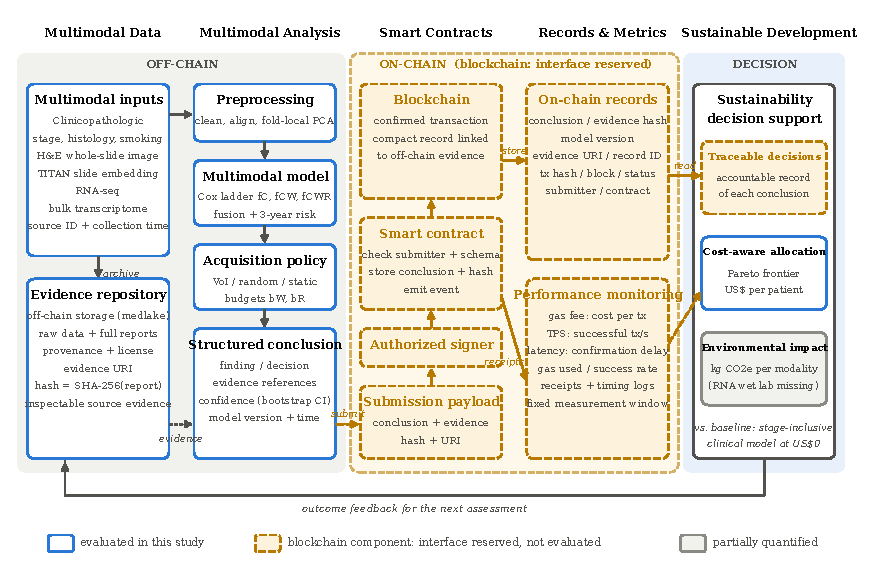
\includegraphics[width=\textwidth]{fig0_architecture.pdf}
\caption{Model-evidence registration. Frozen B1 outputs pass through the ledger adapter to a Solidity registry on Ethereum Sepolia. Protocol and result files remain in the evidence repository; the contract stores their commitment, aggregate conclusions and version information. Auditing combines file-hash verification with contract records and transaction metrics.}
\label{fig:arch}
\end{figure*}

%====================================================================
\section{Related Work}
\subsection{Multimodal Survival Prediction and Benchmarks}
Fusion of histology and genomics improved pan-cancer prognostication over single modalities in several studies~\cite{chen2022,cheerla2019,valesilva2021}. SurvBoard standardized multi-omics survival benchmarking across 28 cancer datasets, including clinical comparators and missing modalities~\cite{wissel2025}. The MMIST-LUNG release, which we use, curated TCGA and CPTAC lung cancer cases with clinical, WSI, transcriptomic, CT and PET data and non-uniform missingness~\cite{mendes_mmist}. These works mostly assume complete acquisition at test time. Our results suggest that the information content of the clinical baseline at the chosen prediction time is decisive for the size of the multimodal gain.

\subsection{Cost-Aware and Dynamic Feature Acquisition}
Acquiring features sequentially under a budget is well studied in machine learning~\cite{ji2007,shim2018,covert2023}. Most methods target classification and estimate the value of the next feature by its expected information gain or loss reduction. SAGEAgent applies agent-based acquisition to multimodal survival prediction and uses the probability of a risk change as an acquisition signal~\cite{qu2026}. We use a deliberately simple VoI proxy, the predicted change in 3-year risk, and ask whether it beats random selection when the baseline is strong; Section~\ref{sec:voi-theory} states when such a proxy is justified.

\subsection{Evaluation of Survival Discrimination}
Uno's IPCW C-index~\cite{uno2011} is the standard truncated concordance measure; implementation choices and transformations of risk predictions can change C-index values substantially~\cite{sonabend2022}. We quantify the effect of retaining patients followed beyond the truncation time in our pipeline.

\subsection{Sustainability of Digital Pathology and Genomics}
Recent analyses quantify the operational cost of clinical-scale digital pathology~\cite{ardon2023}, its greenhouse-gas emissions~\cite{tilmant2026,vafaeisadr2024}, the micro-costs of clinical sequencing~\cite{altburger2026,cuppen2022,kumar2022}, and the carbon footprint of bioinformatic analysis~\cite{grealey2022}. We connect these figures to the predictive value of the modalities they price.

\subsection{Ethereum for Model Evidence}
Ethereum smart contracts store application state at a public address and enforce update rules through transactions~\cite{ethereumcontracts}. MedRec used blockchain metadata for medical-record access and permissions while retaining records in providers' storage~\cite{azaria2016}. We use Ethereum to bind each aggregate model conclusion to a fixed evidence commitment, with separately versioned display metadata. Sepolia provides the test network for deploying and inspecting this registry~\cite{ethereumnetworks}.

%====================================================================
\section{System Architecture}
\label{sec:arch}
The registry connects frozen B1 model outputs to Ethereum through the existing ledger adapter (Fig.~\ref{fig:arch}). Each stage setting produces one aggregate \texttt{ANALYSIS\_RECORD}. The protocol and result files stay in the evidence repository, with a SHA-256 checksum for every file. Their manifest is committed as a single evidence hash.

The Solidity contract stores the fields in Table~\ref{tab:iface}. An owner or authorized submitter registers a record; the contract checks field bounds and the record key against the source ID, then recomputes the analysis digest. Duplicate record IDs are rejected. The conclusion, evidence URI and analysis commitments remain fixed after registration. The owner or an authorized original submitter can revise the display name and description, incrementing the metadata version and emitting an event with the old and new metadata hashes. The model-specification digest covers the supplied protocol and code checksums.

An auditor reconstructs the stored conclusion and recomputes the evidence commitment from the repository files. The adapter accepts aggregate analysis fields and rejects patient identifiers, salts and feature values. Transaction receipts provide gas and block information, while client logs provide submission and receipt-observation times. These records link the cost-performance analysis to its registered version.

\begin{table}[t]
\centering
\caption{Model-Evidence Fields Stored by the Ethereum Registry}
\label{tab:iface}
\setlength{\tabcolsep}{3pt}
\begin{tabular}{@{}>{\raggedright}p{1.9cm}>{\raggedright\arraybackslash}p{6.15cm}@{}}
\toprule
Field group & Stored content \\
\midrule
Identity & Record key and source record ID \\
Analysis & Conclusion ($\le$512 UTF-8 bytes), model version and confidence statement \\
Commitments & Evidence, model-specification and analysis digests \\
Evidence pointer & Repository URI \\
Display metadata & Data name, description, metadata hash and revision version \\
Provenance & Submitter address and creation timestamp \\
\bottomrule
\end{tabular}
\end{table}

%====================================================================
\section{Problem Formulation}
\label{sec:problem}
\subsection{Prediction Task and Estimand}
For patient $i$ let $T_i$ be overall survival time from the GDC index date, $C_i$ the censoring time, and $\tau = 1095$ days. Modalities are acquired in a fixed order $m \in \{0,1,2\}$: clinicopathologic data including pathologic stage ($X^{(0)}$), plus WSI ($X^{(1)}$), plus RNA ($X^{(2)}$). Because WSI and RNA come from resection specimens and pathologic stage is available after surgery, the prediction time point is postoperative. The model at level $m$ outputs a 3-year event probability $r^{(m)}_i = 1 - \hat S_m(\tau \mid X^{(0)}_i,\dots,X^{(m)}_i)$, so that patients scored at different levels can be ranked on one scale. The estimand is the 3-year Uno C-index of the resulting risk vector in the target population, together with the expected incremental acquisition cost per patient.

\subsection{Acquisition Policies}
A policy is defined by budgets $b_W, b_R \in \{0, 0.1, \dots, 1\}$ with $b_R \le b_W$ (66 pairs) and two scores $s_W, s_R$. The top-$b_W$ fraction of patients by $s_W$ receives WSI; among them, the top fraction $b_R$ of all patients by $s_R$ receives RNA. Each patient keeps the risk of the highest level acquired:
\begin{equation}
r_i = \begin{cases} r^{(2)}_i & i \in \mathcal{R},\\ r^{(1)}_i & i \in \mathcal{W}\setminus\mathcal{R},\\ r^{(0)}_i & \text{otherwise,}\end{cases}
\end{equation}
with expected cost per patient $c(b_W, b_R) = b_W c_W + b_R c_R$.

\subsection{Why Predicted Risk Change Is a Reasonable VoI Proxy}
\label{sec:voi-theory}
Let $Y = \mathbb{1}\{T \le \tau\}$ (ignoring censoring for this argument), $p_0 = P(Y{=}1 \mid X^{(0)})$ and $p_1 = P(Y{=}1 \mid X^{(0)}, X^{(1)})$. Since $(Y-p_0)^2-(Y-p_1)^2 = (p_1-p_0)(2Y-p_0-p_1)$ and $E[Y \mid X^{(0)},X^{(1)}] = p_1$,
\begin{equation}
E\big[(Y-p_0)^2-(Y-p_1)^2 \,\big|\, X^{(0)}\big] = E\big[(p_1-p_0)^2 \,\big|\, X^{(0)}\big].
\end{equation}
The expected reduction in Brier loss~\cite{brier1950} therefore equals the expected squared risk change when both models are calibrated conditional probabilities. We use predicted absolute risk change as a ranking proxy. Its relation to the non-decomposable C-index is indirect.

%====================================================================
\section{Materials and Methods}
\label{sec:methods}
Reporting follows TRIPOD~\cite{collins2015} where applicable.

\subsection{Cohort}
We used the MMIST-LUNG curation~\cite{mendes_mmist} of TCGA-LUAD, TCGA-LUSC, CPTAC-LUAD and CPTAC-LSCC~\cite{tcga_luad,tcga_lusc,gillette2020,satpathy2021}. Overall survival was reconstructed from GDC case records using explicit vital status and positive follow-up or death times; deaths without a valid time were never treated as censored. Of 1,365 patients, 52 were excluded (39 with unknown status or death without a valid time, 11 alive without positive follow-up, 2 without a local GDC record). Table~\ref{tab:cohort} summarizes the 1,313 analyzed patients. Pathologic stage groups were reconstructed from the raw GDC diagnoses with the same rules used for the external cohorts; 12 missing values were kept as a separate category.

\begin{table}[t]
\centering
\caption{Analysis Cohort}
\label{tab:cohort}
\setlength{\tabcolsep}{4pt}
\begin{tabular}{@{}lrrr@{}}
\toprule
 & TCGA & CPTAC & Total \\
\midrule
Patients & 1,005 & 308 & 1,313 \\
\quad LUAD / squamous & 509 / 496 & 206 / 102 & 715 / 598 \\
Deaths & 397 & 87 & 484 \\
With WSI features & 1,005 & 305 & 1,310 \\
With RNA features & 997 & 308 & 1,305 \\
\midrule
\multicolumn{4}{@{}l}{Pathologic stage: I 666, II 371, III 230, IV 34, missing 12} \\
\multicolumn{4}{@{}l}{Median observed time: 669 days} \\
\bottomrule
\end{tabular}
\end{table}

\subsection{Modalities and Features}
\textit{Clinicopathologic (level 0):} ten-year age bin, sex, race, ethnicity, smoking status, pack-years and smoking years, ICD-10 code, morphology, prior malignancy, and pathologic stage group (I--IV). A contrast analysis removes stage. \textit{WSI (level 1):} author-provided 768-dimensional TITAN slide embeddings~\cite{titan}, averaged per patient (4,532 slides). \textit{RNA (level 2):} author-provided bulk transcriptome features (10,270 features). Within each training fold, the WSI and RNA blocks were reduced by keeping the 256 highest-variance features, standardizing and projecting onto 16 principal components. CT and PET features were available for only 68 and 30 patients and were not used.

\subsection{Prognostic Models}
Within each of five outer folds (stratified by source and event; seed 20261004), we fitted three Breslow Cox models with a ridge penalty $\alpha \in \{1, 10, 100\}$ selected by Harrell's C on an inner 20\% validation split~\cite{polsterl2020}: $f_C$ (clinicopathologic), $f_{CW}$ (adding the WSI block and a presence indicator) and $f_{CWR}$ (adding the RNA block and indicator). Patients lacking a modality (3 for WSI, 8 for RNA) were handled through the presence indicators. Each test fold held about 263 patients.

\subsection{Acquisition Policies}
\textit{VoI policy.} Training targets were the absolute risk changes $d_W = |r_{CW} - r_C|$ and $d_R = |r_{CWR} - r_{CW}|$, obtained on the outer training set by inner five-fold cross-fitting, with all three Cox models refitted in each inner fold. Gradient-boosted regressors (depth 3, learning rate 0.05, 200 iterations) predicted $d_W$ from level-0 features and $d_R$ from level-0 plus WSI features. \textit{Random policy:} the same budgets, averaged over 100 random selections per fold. \textit{Static policies:} the corners of the grid. \textit{Risk-change oracle:} ranks test patients by their true $d$, i.e.\ by how much the fuller model would move their risk. It is a diagnostic reference for the VoI regressor, not an upper bound on attainable discrimination, because a large risk change need not improve the ranking.

\subsection{Cost Vector}
Costs are incremental to standard care (Table~\ref{tab:cost}). For WSI we summed scanner ownership (US\$0.55--19.53 per slide), scanning staff (US\$0.79--0.92) and on-premise storage (2\,GB per slide at US\$1\,M per petabyte including redundancy, i.e.\ US\$2.00) from a clinical-scale operation~\cite{ardon2023}, and multiplied by the observed 3.46 slides per patient. For RNA sequencing we used a lower bound of WTS consumables (\texteuro278 per case~\cite{altburger2026}; US\$300 at an assumed 1.08\,US\$/\texteuro) and an upper bound of a clinical whole-exome/whole-transcriptome test (US\$2,919~\cite{ortendahl2025}). Two scenarios span the plausible cost ratio: \emph{low ratio} (WSI \$78, RNA \$300; $\kappa = 3.9$) and \emph{high ratio} (WSI \$12, RNA \$2,919; $\kappa \approx 253$, using unrounded costs). Because policies are defined by acquisition fractions, any other cost vector maps onto the same results without refitting. These are scenario values from the literature, not measured costs in our setting; if RNA or scanning is already performed for another clinical purpose, its incremental prognostic cost is zero.

\begin{table}[t]
\centering
\caption{Incremental Acquisition Cost Vector per Patient}
\label{tab:cost}
\setlength{\tabcolsep}{3pt}
\begin{tabular}{@{}>{\raggedright\arraybackslash}p{1.5cm}>{\raggedright\arraybackslash}p{3.1cm}>{\raggedright\arraybackslash}p{3.15cm}@{}}
\toprule
 & H\&E WSI & RNA sequencing \\
\midrule
Monetary (US\$) & 11.6--77.7 (3.34--22.45 per slide $\times$ 3.46 slides)~\cite{ardon2023} & 300 (consumables only)~\cite{altburger2026} to 2,919 (clinical WES/WTS)~\cite{ortendahl2025} \\
Turnaround & $\approx$1 min scanning per slide (modelling assumption); same day~\cite{vafaeisadr2024} & $<$10--14 working days (WGTS)~\cite{cuppen2022} \\
Carbon (kg CO$_2$e) & 0.25--0.35 (0.073--0.101 per slide incl.\ 1-year storage; French grid)~\cite{tilmant2026} & $\ge$0.05--5 (alignment compute only, 50\,M reads)~\cite{grealey2022}; wet lab not quantified \\
\bottomrule
\end{tabular}
\end{table}

\subsection{Evaluation and Statistics}
The primary metric was the 3-year Uno IPCW C-index~\cite{uno2011}, with the censoring distribution estimated on the outer training set and patients with $t \ge \tau$ retained as comparators, averaged over folds. Our matrix implementation matched scikit-survival to within $10^{-10}$, including on bootstrap resamples. Secondary metrics were the 3-year cumulative/dynamic AUC and IPCW Brier score. Uncertainty used a paired bootstrap of test patients within folds (2,000 replicates, seed 20261008; 500 for off-diagonal grid points); all policies shared the same resamples, and fold-wise differences were averaged before taking percentiles. Intervals condition on the fitted models.

Four questions were prespecified. Q1 asked for the smallest RNA budget $b_R^*$ (with WSI for all) whose difference from RNA-for-all had a 95\% lower bound above $-\delta$, with $\delta = 0.01$. Q2 compared VoI with random selection at $b_R \in \{0.1, 0.2, 0.3, 0.5\}$ with Holm correction. Q3 computed cost-performance frontiers. Q4 repeated everything without stage. A depth-2 decision tree was prespecified to summarize which patients the VoI policy selects at $b_R^*$.

\subsection{External Transportability of the RNA Branch}
In a separately frozen analysis, a single RNA\,+\,clinical Cox model was trained on the development cohort (GDC STAR-Counts TPM, 10,902 genes shared with all platforms, within-sample rank normalization) and applied unchanged to seven GEO microarray cohorts~\cite{edgar2002} on four platforms (1,690 patients, 718 deaths). Cohort-level differences were pooled by DerSimonian--Laird random effects~\cite{dersimonian1986}.

\subsection{Reproducibility}
The clinical-analysis protocol was frozen with a SHA-256 record before any policy was run, and the analysis script verifies that hash at run time; there were no deviations from that protocol. The analysis ran on CPU only. The registry experiment reused its frozen aggregate outputs.

\subsection{Registry Evaluation}
\label{sec:chain-methods}
The registry used the two frozen B1 conclusions, one for each stage setting. Its evidence bundle contained the protocol, freeze record, result JSON, two grid-mean CSV files and report. The bundle commitment preserved the native encoding: SHA-256 of Python's default JSON serialization of sorted (relative path, file SHA-256) pairs. Functional checks covered authorization, duplicate submission, record reconstruction, analysis-digest validation and display-metadata revision. The auditor also checked 128 single-bit mutations of the commitment preimage. Contract tests included two fuzz properties with 256 cases each.

For the local overhead comparison, each backend received three repetitions of 16 writes in each of two display-payload classes: 16/64 and 128/512 UTF-8 bytes for name/description, respectively (96 writes per backend). The analysis schema was held fixed and backend order alternated across repetitions. The comparator was an EIP-191-signed, SHA-256 hash-chained JSONL log, flushed with \texttt{fsync} after each append. Runs used an Apple M3 (8 logical CPUs, 16 GiB RAM), Node 25.2.1, ethers 6.17.0 and Foundry/Anvil 1.7.1. The contract was compiled with Solidity 0.8.34, optimizer 200 runs and a Shanghai target. Anvil used chain ID 31337, 1-s blocks and a 30-million-gas block limit. EVM writes ran in batches of four with 100-ms receipt polling; the log appended sequentially. Latency ended at observation of a successful one-confirmation receipt or completion of a signed, flushed append. Observed write rate was completed writes divided by elapsed time from the first submission to the last completion.

The public deployment used Ethereum Sepolia (chain ID 11155111) and a dedicated account. The four successful operations were deployment, two registrations and one description revision. Each gas limit was estimated on the live network with 20\% headroom. Gas used and effective gas price came from receipts; their product gave the actual fee. Block timestamps came from the corresponding canonical block headers, and client logs supplied submission times and one-confirmation receipt latency.


%====================================================================
\section{Results}
\subsection{Static Policies}
With stage, the clinicopathologic model achieved a 3-year C-index of 0.644 (95\% CI 0.617--0.673), WSI for all 0.638 (0.610--0.667) and WSI\,+\,RNA for all 0.645 (0.618--0.674) (Fig.~\ref{fig:static}). Without stage the corresponding values were 0.580 (0.550--0.607), 0.610 (0.582--0.639) and 0.622 (0.596--0.650). WSI therefore contributed $+0.030$ and RNA a further $+0.012$ only when the baseline lacked stage.

\begin{figure}[t]
\centering
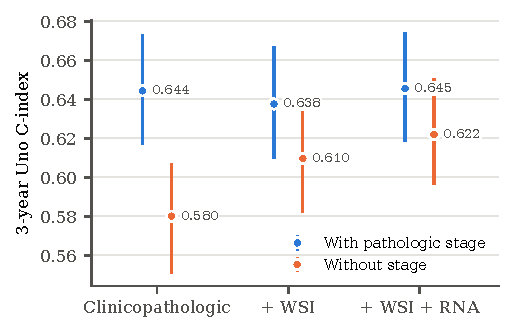
\includegraphics[width=\columnwidth]{fig2_static.pdf}
\caption{Static policies: 3-year Uno C-index (5-fold mean, 95\% bootstrap CI) for the three acquisition levels, with and without pathologic stage in the clinical baseline.}
\label{fig:static}
\end{figure}

\subsection{How Much RNA Sequencing Is Needed (Q1)}
Table~\ref{tab:q1} lists the differences from RNA-for-all. Across all budgets the point difference lay between $-0.008$ and $+0.001$ with stage and between $-0.012$ and $+0.001$ without (Fig.~\ref{fig:ni}). The prespecified rule returned $b_R^* = 0.8$ in both settings. The selected budget was driven by interval width. At low budgets the 95\% interval half-width ($\approx$0.02 with about 263 test patients per fold) exceeds $\delta$, whereas intervals narrow mechanically as the policy converges to RNA-for-all. The prespecified decision tree, trained to reproduce the top-80\% selection, predicted ``acquire'' in every leaf in all folds and yielded no discriminating rule. At low budgets, the intervals still allowed C-index losses of about 0.02.

\begin{table}[t]
\centering
\caption{Q1: Difference in 3-Year C-Index from RNA Sequencing for All (WSI for All)}
\label{tab:q1}
\setlength{\tabcolsep}{4pt}
\begin{tabular}{@{}lll@{}}
\toprule
$b_R$ & With stage & Without stage \\
\midrule
0.0 & $-0.008$ ($-0.026$, 0.010) & $-0.012$ ($-0.034$, 0.007) \\
0.1 & $+0.000$ ($-0.017$, 0.018) & $-0.006$ ($-0.026$, 0.013) \\
0.2 & $-0.006$ ($-0.023$, 0.011) & $+0.001$ ($-0.017$, 0.019) \\
0.3 & $-0.006$ ($-0.021$, 0.010) & $-0.004$ ($-0.021$, 0.013) \\
0.5 & $-0.007$ ($-0.019$, 0.005) & $-0.001$ ($-0.016$, 0.013) \\
0.7 & $-0.004$ ($-0.012$, 0.004) & $-0.001$ ($-0.011$, 0.009) \\
0.8 & $-0.002$ ($-0.008$, 0.004)$^{*}$ & $-0.001$ ($-0.008$, 0.007)$^{*}$ \\
0.9 & $+0.001$ ($-0.003$, 0.005) & $-0.002$ ($-0.007$, 0.003) \\
\bottomrule
\multicolumn{3}{@{}l}{\footnotesize $^{*}$Smallest budget meeting the prespecified criterion ($b_R^*$).}
\end{tabular}
\end{table}

\begin{figure*}[t]
\centering
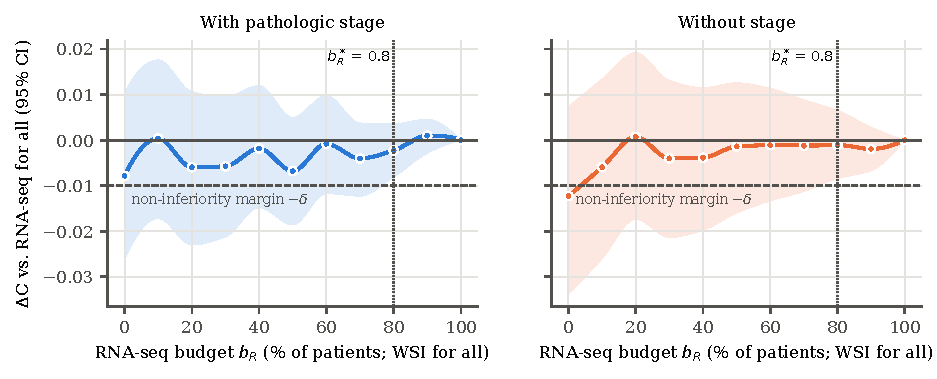
\includegraphics[width=0.85\textwidth]{fig3_noninferiority.pdf}
\caption{Q1. Difference in 3-year C-index between the VoI policy at RNA budget $b_R$ (WSI for all) and RNA sequencing for all, with 95\% paired-bootstrap CI. Dashed: margin $-\delta = -0.01$. Dotted: $b_R^*$. No budget shows a detectable loss; $b_R^*$ is driven by interval width.}
\label{fig:ni}
\end{figure*}

\subsection{VoI Versus Random Selection (Q2)}
The VoI regressors predicted the realized risk change only weakly: test-set Spearman $\rho$ was 0.18--0.36 for the RNA step and $-0.03$ to 0.25 for the WSI step across folds and settings. With stage, VoI exceeded random selection at $b_R = 0.1$ by $+0.008$ (95\% CI 0.001--0.015; raw $p = 0.021$, Holm $p = 0.084$) and was indistinguishable at 0.2, 0.3 and 0.5. Without stage, the largest difference was $+0.011$ at $b_R = 0.2$ (0.001--0.020; raw $p = 0.030$, Holm $p = 0.12$) (Fig.~\ref{fig:voi}). No comparison survived correction. The risk-change oracle exceeded random selection by at most about 0.016 C-index.

\begin{figure*}[t]
\centering
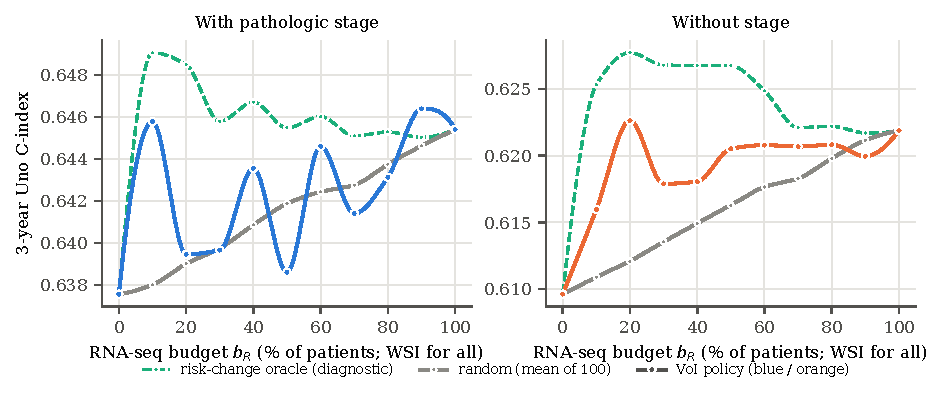
\includegraphics[width=0.85\textwidth]{fig5_voi_vs_random.pdf}
\caption{Q2. 3-year C-index of VoI, random (mean of 100 draws) and risk-change-oracle selection versus RNA budget, with WSI acquired for all patients. The oracle ranks patients by their realized risk change.}
\label{fig:voi}
\end{figure*}

\subsection{Cost-Performance Frontiers (Q3, Q4)}
The zero-cost policy is the cheapest point and therefore always on the frontier; the informative question is whether any costlier point improves on it. With stage, only two such points existed in both cost scenarios ($b_W = 0.5$ or $0.6$ with $b_R = 0.1$), with C-index 0.647 and 0.650, i.e.\ $+0.003$ and $+0.006$ above the zero-cost policy and well inside its interval (0.617--0.673) (Table~\ref{tab:pareto}, Fig.~\ref{fig:pareto}, top). Their expected cost was US\$69--77 per patient in the low-ratio and US\$298--299 in the high-ratio scenario. Without stage, the frontier rose along the WSI axis first, reaching 0.610 with WSI for all at US\$12--78 per patient, and admitted RNA only afterwards: 0.616 at $b_R = 0.1$ and 0.623 at $b_R = 0.2$, at US\$108--138 (low ratio) or US\$304--595 (high ratio) per patient (Fig.~\ref{fig:pareto}, bottom). Secondary metrics were flat across RNA budgets with stage (3-year AUC 0.682--0.692; Brier 0.208--0.211) and without stage (AUC 0.649--0.663; Brier 0.215--0.220).

\begin{table}[t]
\centering
\caption{Frontier Points Above the Zero-Cost Policy}
\label{tab:pareto}
\setlength{\tabcolsep}{3.5pt}
\begin{tabular}{@{}llrrl@{}}
\toprule
Baseline & ($b_W$, $b_R$) & \multicolumn{2}{c}{US\$/patient} & C-index (95\% CI) \\
 & & low & high & \\
\midrule
With stage & (0, 0) & 0 & 0 & 0.644 (0.617, 0.673) \\
 & (0.5, 0.1) & 69 & 298 & 0.647 (0.619, 0.675) \\
 & (0.6, 0.1) & 77 & 299 & 0.650 (0.624, 0.681) \\
\midrule
Without stage & (0, 0) & 0 & 0 & 0.580 (0.550, 0.607) \\
 & (1, 0) & 78 & 12 & 0.610 (0.582, 0.639) \\
 & (1, 0.1) & 108 & 304 & 0.616 (0.590, 0.646) \\
 & (1, 0.2) & 138 & 595 & 0.623 (0.597, 0.654) \\
\bottomrule
\multicolumn{5}{@{}>{\raggedright\arraybackslash}p{8.4cm}@{}}{\footnotesize Without stage, intermediate WSI-only frontier points are omitted. Low/high: low and high RNA:WSI cost-ratio scenarios (Table~\ref{tab:cost}).}
\end{tabular}
\end{table}

\begin{figure*}[t]
\centering
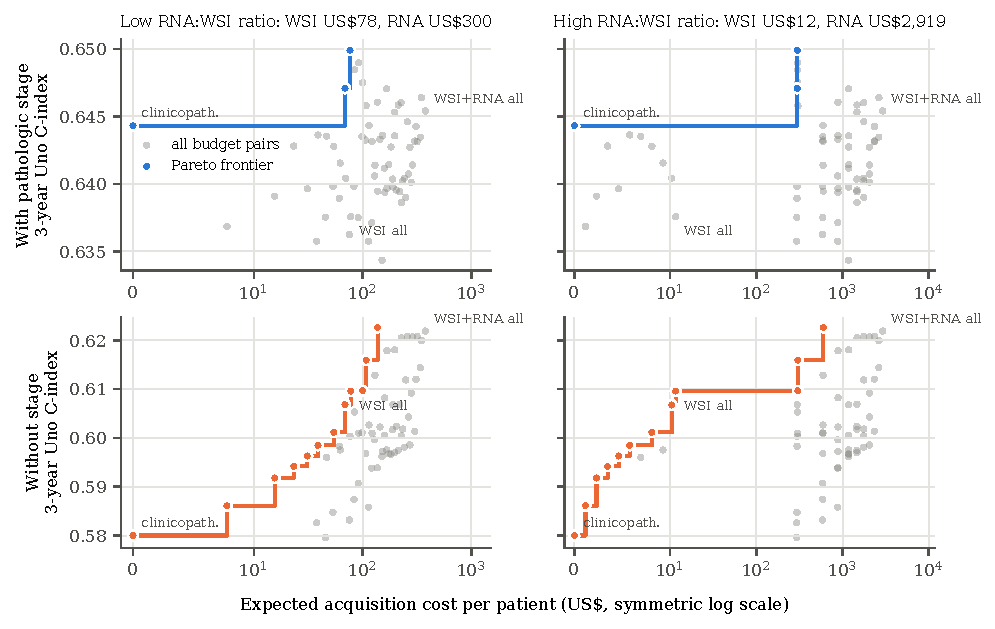
\includegraphics[width=0.92\textwidth]{fig4_pareto_usd.pdf}
\caption{Q3/Q4. Cost-performance frontiers in US dollars per patient for the 66 budget pairs (gray) under low and high RNA:WSI cost ratios (Table~\ref{tab:cost}). Top: baseline with pathologic stage; bottom: without stage. Points above the zero-cost policy in the top row lie within its bootstrap interval.}
\label{fig:pareto}
\end{figure*}

\subsection{Stage Attenuation Internally and Externally}
Against a stage-free clinical baseline, full WSI\,+\,RNA fusion gained $+0.042$ (95\% CI 0.008--0.077; $p = 0.012$) internally. With stage the gain was $+0.001$ ($-0.024$ to 0.029; $p = 0.96$), and with the full prespecified TNM coding $+0.004$ ($-0.019$ to 0.029). In the seven external GEO cohorts the RNA branch gained $+0.073$ (0.043--0.103; $I^2 = 0.25$) without and $+0.022$ ($-0.001$ to 0.045; $I^2 = 0.41$) with stage; six of seven cohort estimates were positive with stage (Fig.~\ref{fig:forest}).

\begin{figure}[t]
\centering
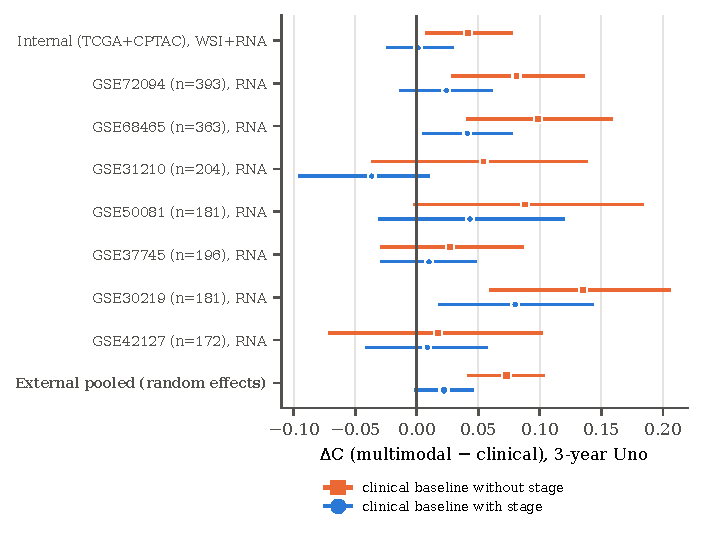
\includegraphics[width=\columnwidth]{fig6_stage_attenuation.pdf}
\caption{Attenuation of multimodal gains when pathologic stage enters the clinical baseline. Internal: WSI\,+\,RNA fusion in TCGA+CPTAC (5-fold). External: RNA\,+\,clinical model trained once on the development cohort and applied to seven GEO cohorts; pooled by random effects.}
\label{fig:forest}
\end{figure}

\subsection{Sensitivity to the IPCW Implementation}
An implementation we had used in an earlier stage of this project discarded test patients followed beyond $\tau$ before computing concordance, instead of retaining them as comparators as in Uno's estimator. It reported the internal stage-free fusion gain as $+0.071$ (0.031--0.108) instead of $+0.042$, an inflation of about 70\%, because the excluded long-term survivors are the most informative comparators for early events. With stage, the same implementation gave $+0.022$ ($-0.007$ to 0.051), leading to the same qualitative conclusion.

\subsection{Evidence Registration and Write Overhead}
\label{sec:chain-results}
Both B1 conclusions were registered and reconstructed with the original evidence commitment. All 30 contract tests and nine native-adapter checks passed, and all 128 altered commitment preimages were rejected. Replaying identical records reused the existing receipts. A description revision preserved the evidence, model-specification and analysis digests.

Local deployment used 1,428,475 gas; registering the two B1 records used 682,909 and 682,825 gas, and revising one description used 61,528 gas. Longer display metadata increased registration gas in the synthetic workload (Table~\ref{tab:registry}). The signed log completed writes more quickly under the tested configuration. Modified entries were detected; truncation was detected when the verifier held a trusted head checkpoint.

On Sepolia, deployment, both registrations and the description revision produced four successful receipts. Table~\ref{tab:sepolia} reports the gas, fees and timing of each operation. The registered evidence commitment matched the original files after the revision.

\begin{table*}[t]
\centering
\caption{Local registry overhead: three repetitions of 16 writes per backend and payload class}
\label{tab:registry}
\setlength{\tabcolsep}{7pt}
\begin{tabular}{@{}llrrr@{}}
\toprule
Backend & Display payload & Gas per registration & Receipt / append latency (ms) & Observed writes/s (range) \\
\midrule
Local EVM & compact & 476,930 & 982.34 & 4.21 (3.99--4.33) \\
Local EVM & extended & 889,876 & 967.13 & 4.13 (4.04--4.24) \\
Signed log & compact & -- & 3.98 & 249.29 (243.18--353.30) \\
Signed log & extended & -- & 3.03 & 348.75 (299.98--359.10) \\
\bottomrule
\end{tabular}
\par\smallskip
\begin{minipage}{0.96\textwidth}\footnotesize
Gas and latency are medians of the three within-repetition medians; write rates are medians with the repetition range in parentheses. Compact/extended payloads use 16/64 and 128/512 name/description bytes. The EVM used 1-s blocks and four outstanding writes; the log appended sequentially with signing and \texttt{fsync}. Rates describe these client configurations and completion endpoints.
\end{minipage}
\end{table*}

\begin{table*}[t]
\centering
\caption{Gas, fees and timing of four successful Sepolia transactions on 22 October 2026 (UTC)}
\label{tab:sepolia}
\small
\setlength{\tabcolsep}{4pt}
\begin{tabular}{@{}lrrrccr@{}}
\toprule
Operation & Block & Gas used & \shortstack{Fee ($10^{-9}$\\SepoliaETH)} & \shortstack{Submission\\start (UTC)} & \shortstack{Block time\\(UTC)} & \shortstack{Receipt\\latency (s)} \\
\midrule
Deployment & 11,967,396 & 9,986,101 & 13.141708916 & 05:14:56.284 & 05:15:12 & 19.59 \\
Stage-inclusive record & 11,967,397 & 3,139,469 & 4.131541204 & 05:15:17.461 & 05:15:24 & 7.89 \\
Stage-excluded record & 11,967,398 & 3,139,385 & 4.131430660 & 05:15:26.884 & 05:15:36 & 13.34 \\
Metadata revision & 11,967,399 & 191,886 & 0.252521976 & 05:15:42.516 & 05:15:48 & 7.31 \\
\midrule
Total & -- & 16,456,841 & 21.657202756 & -- & -- & -- \\
\bottomrule
\end{tabular}
\par\smallskip
\begin{minipage}{0.98\textwidth}\footnotesize
All receipts had status 1 on chain ID 11155111. Effective gas price was 1,316 wei/gas for all four transactions; fee equals gas used times this price. The total was $0.000000021657202756$ SepoliaETH. Submission start and receipt latency came from the client log; block time is the inclusion-block timestamp. Latency ended at observation of a one-confirmation receipt. Full hashes and unrounded values appear in the supplied transaction CSV. Contract: \href{https://sepolia.etherscan.io/address/0xF3A2732f7521ED01A0AeaB874F9b2E46aB6B0155}{\texttt{0xF3A2732f7521ED01A0AeaB874F9b2E46aB6B0155}}.
\end{minipage}
\end{table*}


%====================================================================
\section{Discussion}
\subsection{Principal Findings}
In postoperative NSCLC prognostication with a stage-inclusive baseline, neither digitized histology nor bulk transcriptomics added detectable discrimination in this cohort, and no costlier acquisition policy improved on the policy that uses only information routine pathology already produces. Per-patient VoI selection could not identify a subgroup for which RNA sequencing was worth its cost. Without stage, the picture changed: WSI then carried much of the missing information at a cost one to two orders of magnitude below RNA sequencing and entered the frontier first.

\subsection{Relation to Prior Work}
SAGEAgent~\cite{qu2026} and our policy both use risk change to guide acquisition, although their disease, modality and baseline settings differ. Section~\ref{sec:voi-theory} links squared risk change to expected Brier-loss reduction under calibration; the weak fold-wise Spearman correlations indicate that predicting this signal before acquisition was difficult in our setting. SurvBoard~\cite{wissel2025} includes clinical comparators in multi-omics benchmarking. Our results show how adding stage to that comparator changes both the multimodal gain and the cost-performance frontier.

\subsection{Implications for Evaluation}
A fusion gain measured against a stage-free baseline in a postoperative setting partly re-discovers stage, and an implementation detail of the IPCW C-index can inflate it further. We recommend that such studies state the prediction time point and include all information available at that time in the clinical baseline, use and report the exact concordance estimator, and report acquisition costs alongside discrimination, preferably as frontiers that readers can re-price with their own costs.

\subsection{Implications for Sustainable Health Systems}
Routine clinicopathology provided a strong postoperative prognostic baseline in this cohort. WSI acquisition offered its clearest incremental value when stage was omitted. RNA sequencing also serves treatment selection, including actionable fusion detection~\cite{ortendahl2025}; when it is already acquired for that purpose, its incremental prognostic cost is zero. Resource planning also depends on storage duration: the WSI carbon estimates are dominated by storage~\cite{tilmant2026}, whereas the RNA estimates in our cost vector cover computation.

\subsection{Role of the Ethereum Registry}
The Ethereum record provides a common reference for the reported conclusion, its supporting file hashes and subsequent label revisions. The analysis history can be retrieved independently of the application's local database. The signed log offered lower write overhead in the local benchmark, so deployment choice depends on who must maintain and verify that history. Scientific review also requires access to the underlying evidence files.

\subsection{Limitations}
Policy analyses used internal cross-validation in one development cohort. CPTAC had contributed to earlier development, so external confirmation is confined to the RNA branch. Incomplete reconciliation of specimen collection and GDC index dates also leaves the postoperative information timing uncertain.

The WSI and RNA inputs were frozen, author-provided representations whose preprocessing and potential overlap with WSI-encoder pretraining could not be fully audited. The observed modality gains therefore apply to these representations and Cox models. At low acquisition budgets, the interval width limited the non-inferiority analysis and largely determined $b_R^*$. The VoI target relies on calibration and tracks risk change only indirectly related to concordance.

Acquisition costs represent literature-derived scenarios from a few health systems; the wet-lab carbon footprint of RNA sequencing remains unquantified. Registry measurements cover two aggregate records and a small synthetic workload, with public-network timing and fees measured for the four Sepolia operations.

\subsection{Future Work}
The stage-attenuation result should next be tested with stronger slide and expression encoders in a cohort with fully documented specimen and outcome timing. Acquisition scores targeting calibrated expected loss reduction would help distinguish limitations of the risk-change proxy from limitations of the available features. For the registry, multiple writers and independently maintained evidence copies would allow evaluation of access, recovery and audit completeness across organizations.

%====================================================================
\section{Conclusion}
After resection, routine clinicopathologic data including stage yielded similar 3-year discrimination to universal WSI and RNA acquisition in this cohort, at zero incremental cost. VoI selection identified no subgroup for which RNA sequencing justified its acquisition cost. Without stage, WSI was the cost-effective first addition. These comparisons depend on prediction-time information and the IPCW estimator. The Ethereum registry links the aggregate conclusions to their evidence commitments and records display-metadata revisions.

\Needspace{10\baselineskip}
\section*{Data and Code Availability}
All data are public (GDC, MMIST-LUNG, GEO). Code, the frozen protocol with its SHA-256 record, fold assignments, aggregate outputs and the Ethereum registry implementation are available at \todo{repository URL}. Contract source and transaction metrics accompany the manuscript; Table~\ref{tab:sepolia} links to the public deployment.

\bibliographystyle{IEEEtran}
\bibliography{refs}

\end{document}
